\documentclass[border=0.5mm]{standalone}

\usepackage{import}
\subimport{../../../}{preamble.tex}

\usepackage{tikz}
\usetikzlibrary{calc}

\usepackage{pgfplots}
\usepgfplotslibrary{fillbetween}

\begin{document}

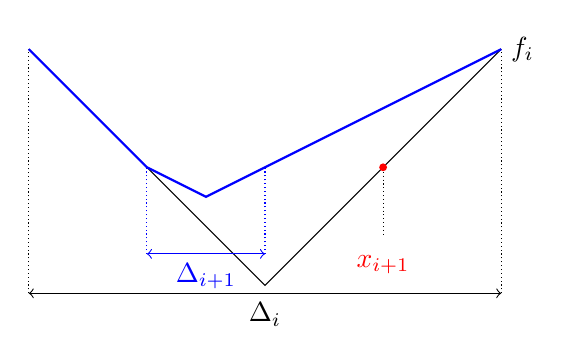
\begin{tikzpicture}

  % The funciton $f_i$
  \draw[black] (-3,3) -- (0,0) -- (3,3);
  \node[right] at (3,3) {$f_i$};

  % The set $\Delta_i$
  \draw[<->, black] (-3,-0.1) -- (3,-0.1);
  \node[below] at (0, -0.1) {$\Delta_i$};
  \draw[densely dotted] (-3, -0.1) -- (-3, 3);
  \draw[densely dotted] (3, -0.1) -- (3, 3);

  % The new evaluation $x_{i+1}$
  \node[circle, inner sep=1, fill=red] (f0) at (1.5, 1.5) {};
  \node(x0) at (1.5, 0.5) {};
  \node[below, red] at (x0) {$x_{i+1}$} {};
  \draw[densely dotted] (f0) -- (x0) ;

  % The funciton $f_{i+1}$
  \draw[blue, thick] (-3,3) -- (-1.5,1.5) -- (-0.75,1.125) -- (0, 1.5) -- (3,3);

  % The set $\Delta_{i+1}$
  \draw[<->, blue] (-1.5, 0.4) -- (0, 0.4);
  \node[below, blue] at (-0.75, 0.4) {$\Delta_{i+1}$};
  \draw[blue, densely dotted] (-1.5, 0.4) -- (-1.5, 1.5);
  \draw[blue, densely dotted] (0, 0.4) -- (0, 1.5);
  
\end{tikzpicture}

\end{document}

%%% Local Variables:
%%% mode: latex
%%% TeX-master: t
%%% End:
